% ---------------------------------------------------------------------------
\section{Hepburn System}\jsec{ヘボン式} \label{sec:Hepburn}
% [o] INDEX
\ifor{Hepburn System}{ヘボン式}{へぼんしき}{Hepburn System}
\ifor{older Hepburn System}{標準ヘボン式ローマ字}{ひょうじゅん・へぼん・ろまあじ}{altes Hepburn System}
\ifor{newer Hepburn System}{修正ヘボン式ローマ字}{しゅうせい・へぼんしき・ろうまじ}{neueres Hepburn System}
\ithree{James Curtis Hepburn}{James Curtis Hepburn}{James Curtis Hepburn}

\begin{tabular}{lr}
\begin{minipage}{10.5cm}

The { ヘボン式} {【へぼんしき】} is one of the two most important transcription
systems for Japanese written \hyperref[sec:Mora]{morae} based language. The
{ヘボン式} is most used system worldwide and in Japan.

The word {ヘボン} (hebon) is an old writing of the name \textbf{Hepburn}, a US
American physician, translator, educator and lay Christian missionary, who used
it his first Japanese English Dictionary (3rd ed.) in 1867.

There are manly two different variants. The older {標準ヘボン式ローマ字}
{【ひょうじゅん・へぼん・ろまあじ】} variant, which is used for signs at train
stations. And the new variant the {修正ヘボン式ローマ字}
{【しゅうせい・へぼんしき・ろうまじ】} which is used as a revised system since
1954 in Kenkyusha dictionaries. Most western scientists are using this system.
This system is also used in this book.

\Link \href{http://en.wikipedia.org/wiki/James_Curtis_Hepburn}{Hepburn}

\end{minipage}
&
\raisebox{-.47\height}{
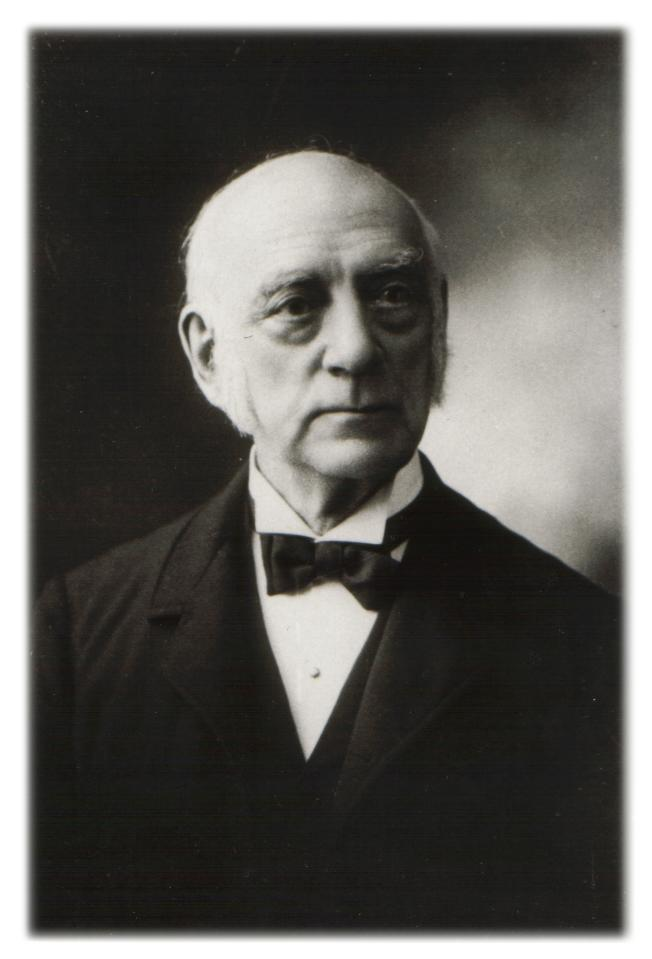
\includegraphics[scale=0.5,trim= 00 00 00 00]{../share/ei/James_Curtis_Hepburn.jpg}}
\\
\end{tabular}


